\subsection{Ca sử dụng đăng ký}
\vspace{0.5cm}


\noindent 
\begin{tabularx}{\linewidth}{| l | X |} 
\hline 
\textbf{Mô tả} & Cho phép người dùng tạo một tài khoản trên ứng dụng để sử dụng các chức năng. \\ 
\hline 
\textbf{Luồng cơ bản} & 1. Người dùng truy cập màn hình đăng ký tài khoản. \newline
                       2. Ứng dụng hiển thị giao diện đăng ký tài khoản, yêu cầu người dùng nhập thông tin. \newline
                       3. Người dùng điền tên, email và mật khẩu của tài khoản muốn đăng ký. \newline
                       4. Người dùng nhấn đăng ký để hoàn thành quá trình. \newline
                       5. Hệ thống kiểm tra thông tin người dùng để trả về thông báo phù hợp và điều hướng người dùng đến màn hình điền thông tin cơ bản. \\ 
\hline 
\textbf{Luồng thay thế} &
                       - Nếu có lỗi tại server, hệ thống sẽ không lưu lại thông tin đã nhập vào. \newline
                       - Nếu thông tin nhập vào không hợp lệ sẽ thông báo lỗi để người dùng nhập lại. \\ 
\hline 
\textbf{Tiền điều kiện} & - Màn hình đăng ký đã hiển thị thành công trên ứng dụng. \newline
                       - Tài khoản email đúng định dạng và chưa được đăng ký trước đây. \\ 
\hline 
\textbf{Hậu điều kiện} & - Người đã đăng ký tài khoản có thể sử dụng nó để đăng nhập và thực hiện các chức năng với quyền hạn tương ứng. \newline
                       - Một hồ sơ người dùng được tạo và có thể được chỉnh sửa. \\ 
\hline 
\textbf{Yêu cầu phi chức năng} & Hệ thống xử lý đăng ký không quá 2s \\ 
\hline 
\end{tabularx}

\vspace{0.8cm}

\noindent 
\begin{tabular}{| c | c |}
    \hline
    \textbf{Biểu đồ hoạt động} & \textbf{Quan hệ} \\ 
    \hline
    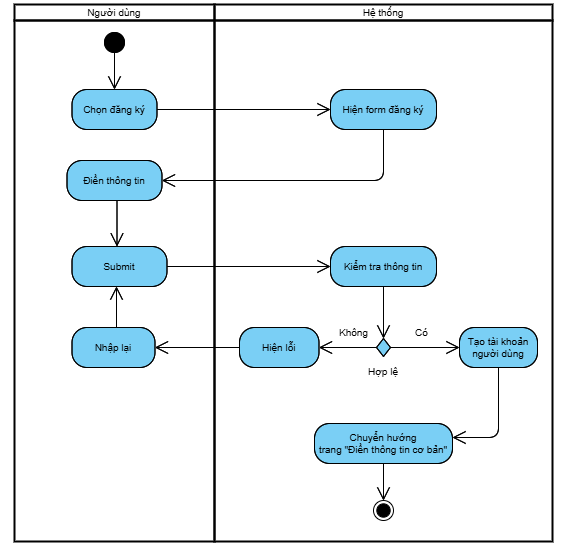
\includegraphics[width=0.6\linewidth]{figures/c3/3-3-2-activity-diagram.png} 
    & 
    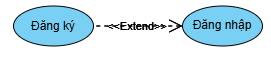
\includegraphics[width=0.35\linewidth]{figures/c3/3-3-2-relationship.png} \\ 
    \hline
\end{tabular}

\begin{figure}[H]
    \centering  
    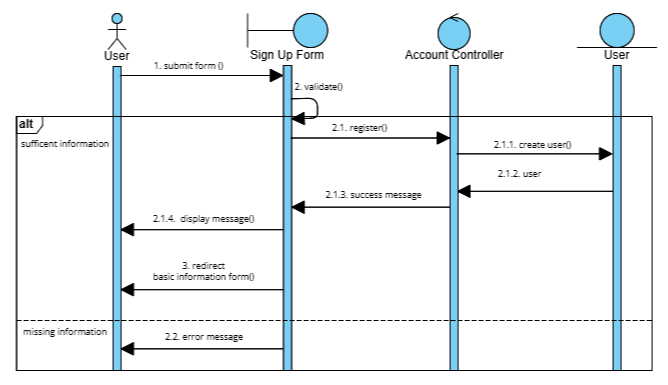
\includegraphics[width=1.1\textwidth]{figures/c3/3-3-2-sequence-diagram.png}
    \caption{Biểu đồ tuần tự ca sử dụng đăng ký.}
    \label{fig:3-3-2-sequence-diagram}
\end{figure}
